
\documentclass[12pt]{article}
\usepackage{times}
\usepackage{setspace}
\setstretch{1.5}
\usepackage{amsmath,amssymb, amsthm}
\usepackage{graphicx}
\usepackage{bm}
\usepackage[hang, flushmargin]{footmisc}
\usepackage[colorlinks=true]{hyperref}
\usepackage[nameinlink]{cleveref}
\usepackage{footnotebackref}
\usepackage{url}
\usepackage{listings}
\usepackage[most]{tcolorbox}
\usepackage{inconsolata}
\usepackage[papersize={8.5in,11in}, margin=1in]{geometry}
\usepackage{float}
\usepackage{caption}
\usepackage{esint}
\usepackage{url}
\usepackage{enumitem}
\usepackage{subfig}
\usepackage{wasysym}
\newcommand{\ilcode}{\texttt}
\usepackage{etoolbox}
\usepackage{physics}
\usepackage{xcolor}
\patchcmd{\thebibliography}{\section*{\refname}}{}{}{}


\makeatletter
\renewcommand{\@seccntformat}[1]{}
\makeatother

\begin{document}



\title{\textbf{CSDS 440: Assignment 4}}

\author{Shaochen (Henry) ZHONG, \ilcode{sxz517} \\ Mingyang TIE, \ilcode{mxt497}}
\date{Due on 09/25/2020, submitted \textcolor{blue}{early} on 09/18/2020}
\maketitle


% % % % % % % % % % % % % % % % % % % % % % % % % % % % % % % % % %
% % % % % % % % % % % % % % % % % % % % % % % % % % % % % % % % % %
% % % % % % % % % % % % % % % % % % % % % % % % % % % % % % % % % %
\section{Problem 15}

Say we have $X$ being a Bernoulli r. v. Let $P(X = 1) = p$ and $P(X = 0) = 1 - p$ we know that its entropy would be:

\begin{align*}
    H(X) &= H_b(p) = -p\log_2(p) - (1-p)\log_2(1-p) \\
    &\Rightarrow H_b'(p) = \log_2(1-p) - \log_2(p)
\end{align*}

Now plot the function.

\begin{figure}[H]
    \centering
    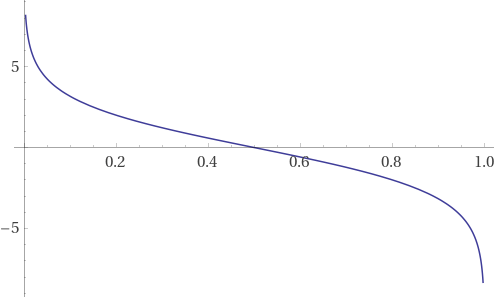
\includegraphics[width=0.4\linewidth]{{fig/fig_p15.png}}
\end{figure}


With the first derivative being a decreasing function, we know the function is concave.



% % % % % % % % % % % % % % % % % % % % % % % % % % % % % % % % % %
% % % % % % % % % % % % % % % % % % % % % % % % % % % % % % % % % %
% % % % % % % % % % % % % % % % % % % % % % % % % % % % % % % % % %
\section{Problem 16}

Pick two points, $x_1$ and $x_2$ in $R^n$ where $Ax_1, Ax_2 \geq b$. W.T.S. for any point $x$ between the line of $x_1$ and $x_2$, we have $Ax \geq b$.

\begin{align*}
    Ax &= A(\lambda x_1 + (1- \lambda)x_2) \\
    &= \lambda A x_1 + (1- \lambda)A x_2 \\
    &\geq \lambda b + (1- \lambda)b = \lambdab + b - \lambda b = b \\
    \Longrightarrow Ax &\geq b
\end{align*}

As $x$ in above case can be any point from of $\{x \mid Ax \geq b \}$, we have proven the set is convex.

% % % % % % % % % % % % % % % % % % % % % % % % % % % % % % % % % %
% % % % % % % % % % % % % % % % % % % % % % % % % % % % % % % % % %
% % % % % % % % % % % % % % % % % % % % % % % % % % % % % % % % % %
\section{Problem 17}

\begin{proof}
To prove by contradiction. Assume we have a local minimum $x$ in a convex function $f$ but there is another global minimum $x'$, where $f(x') < f(x)$.

Since $f$ is convex, by Jensen's inequality we must have:

\begin{align*}
    f(\lambda x + (1 - \lambda)x') &\leq \lambda f(x) + (1 - \lambda)f(x') \\
    &< \lambda f(x) + (1 - \lambda)f(x) \\
    &< f(x) \\
    \text{Let \ } \lambda &= 1 \text{, we will have the below contradiction:} \\
    f(x) &< f(x)
\end{align*}

Thus, by contradiction, the local minimum of a convex function is always the global minimum.

\end{proof}

% % % % % % % % % % % % % % % % % % % % % % % % % % % % % % % % % %
% % % % % % % % % % % % % % % % % % % % % % % % % % % % % % % % % %
% % % % % % % % % % % % % % % % % % % % % % % % % % % % % % % % % %
\section{Problem 18}


% % % % % % % % % % % % % % % % % % % % % % % % % % % % % % % % % %
% % % % % % % % % % % % % % % % % % % % % % % % % % % % % % % % % %
% % % % % % % % % % % % % % % % % % % % % % % % % % % % % % % % % %
% \section{References}
% \nocite{*}
% \raggedright
% \bibliography{references.bib}
% \bibliographystyle{plain}


\end{document}